\subsubsection{Annotation Operations}
\label{sec:geo_annotation_ops}  

Annotations are listed in the 'Annotations' node of the 'Layers' tab. \\

There are two kinds of annotations listed under this node.

\paragraph*{View Point} Annotations provided by an active View Point, e.g. selected evaluation results or externally provided annotation data.
See \ref{sec:key_concepts_viewpoints} for an introductory explanation about View Points. \\

View Point annotations persist as long as the providing View Point is active.

\paragraph*{Grids} Grid data imported into Geographic View. Grid data can be imported into 
Geographic View either by sending it from a Grid View (see \ref{sec:grid_export_geographic}), or via an external GeoTIFF file (see \ref{}). \\

Imported grid items persists in a Geographic View until COMPASS is closed. \\

Clicking on the symbol of the 'Grids' node will open a context menu containing the following operations:

\begin{table}[H]
    \center
    \begin{tabular}{ | l | l |}
      \hline
      \textbf{Operation} & \textbf{Description} \\ \hline
      Remove All & Removes all imported grids from the view \\ \hline
    \end{tabular}
\end{table}

\begin{figure}[H]
    \center
    \hspace*{-2.5cm}
    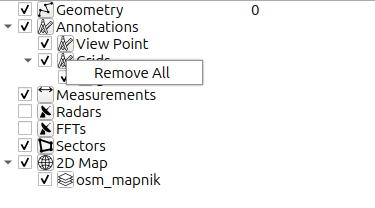
\includegraphics[width=6cm,frame]{figures/geoview_gridops_grids.png}
  \caption{Geographic View 'Grids' node operations}
\end{figure}

Clicking on the symbol of an imported grid item will open a context menu containing the following operations:

\begin{table}[H]
    \center
    \begin{tabular}{ | l | l |}
      \hline
      \textbf{Operation} & \textbf{Description} \\ \hline
      Zoom to Item & Zooms to the grid item \\ \hline
      Rename & Renames the grid item to a specified name \\ \hline
      Export & Exports the grid item to a GeoTIFF file \\ \hline
      Opacity & Sets the opacity of a grid item \\ \hline
      Remove & Removes the grid item from the view \\ \hline
    \end{tabular}
\end{table}

\begin{figure}[H]
    \center
    \hspace*{-2.5cm}
    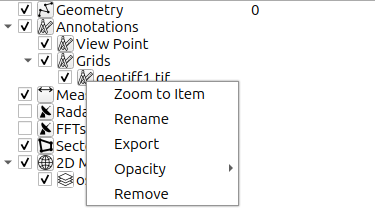
\includegraphics[width=6cm,frame]{figures/geoview_gridops_grid.png}
  \caption{Geographic View grid item operations}
\end{figure}
\ \\

All annotation items can be shown or hidden by using the respective check box next to them.
